\documentclass[a4paper,12pt,oneside,bibtotoc,numbers=noenddot]{scrreprt}

%Pakete
\usepackage[latin9]{inputenc}
\usepackage[ngerman]{babel}
\usepackage{listings}
\usepackage{graphicx}
\usepackage{BachelorThesis}

% Allgemeine Informationen
\newcommand\mytitle{Titel der Arbeit}
\newcommand\myauthor{Name des Autors oder der Autoren}
\newcommand\mydepartment{Informatik und Elektrotechnik}
\newcommand\myinstitute{Hochschule Zittau/G\"{o}rlitz}
\newcommand\mytutor{Name und Titel des betreuenden Professors}
\newcommand\mySecondTutor{Name und Titel des betrieblichen Betreuers}

% Abstracts
\newcommand\mysubject{Das deutsche Abstract.}
\newcommand\mysubjectenglish{The english abstract.}

% PDF-Einstellungen
\hypersetup
{
	pdftitle = \mytitle,
	pdfsubject = \mysubject,
	pdfauthor = \myauthor,
	pdfkeywords = {},
	colorlinks = {true},
	pdfborder = 0 0 0
}

\begin{document}
\nocite{*}

%
\pagenumbering{alph}
\begin{titlepage}
\thispagestyle{empty} 
 \begin{center}
 \vspace{2.0cm} 
 {\bfseries \huge Frontend eines Agilent-Parsers erstellen\\}
 \vspace{3.0cm} 
 {\bfseries \huge Belegarbeit\\}
 \vspace{3.0cm}
 {\normalsize eingereicht am Fachbereich\\}
 {\bfseries \Large Informatik\\}
 {\normalsize der Hochschule Zittau/G�rlitz (HAW)\\}
 \vspace{1cm}
 {\normalsize als Pr�fungsleistung im Fach\\}
 {\bfseries \Large Data Mining 2\\}
 \vspace{1cm}
 {\normalsize vorgelegt von:\\}
 {\bfseries \Large Christof Ochmann (35989)\\
 Ingo K�rner (40586)\\}
 \vspace{1cm}
 {\normalsize  G�rlitz, 07. Februar 2013\\}
 \vspace{0.5cm}
 Betreuer:	Prof. ten Hagen\\
 \vfill
\end{center}
\end{titlepage}

%
%% Kurzreferat
\thispagestyle{empty}
\section*{Abstract}\label{Abstract}
In diesem Projekt...

%\mysubject
%\section*{Abstract}
%\mysubjectenglish

\pagenumbering{Roman}
\tableofcontents
\listoffigures
%\lstlistoflistings

\begin{listofacronyms}
\acronym{JVM}{Java Virtual Machine}

\end{listofacronyms}

\begin{flushleft}
\begin{thebibliography}{sotief}
\bibitem{bib1}{Martin, Robert C. (2008): Clean Code: A Handbook of Agile Software Craftsmanship. Prentice Hall International}

\bibitem{bib2}{Freeman, Eric (2007): Entwurfsmuster von Kopf bis Fu�. O'REILLY}

\bibitem{bib3}{\begin{verbatim}http://www.cs.waikato.ac.nz/ml/weka/arff.html (08.06.2012)\end{verbatim}} 



\end{thebibliography}
\end{flushleft}

\newpage
\pagestyle{chapterStyle}
\pagenumbering{arabic}

\chapter{Allgemeines}
\section{Einleitung}\label{Einleitung}
Ziel dieses Projektes ist es, ...
\section{Aufgabenstellung}\label{Aufgabenstellung}
In diesem Projekt sollen gegebene Agilent-Logdateien geparst werden. Aus den geparsten Zeilen soll ein Baum in einem Intermediate-Format erstellt werden. Der erzeugte Baum wird im Hauptspeicher des Rechners gehalten. Die Weiterverarbeitung des Baumes im Intermediate-Format erfolgt in einem anderen Projekt und ist nicht Gegenstand dieser Arbeit. In diesem Projekt muss das Intermediate-Format nicht entworfen werden. Statt dessen wird es von Felix Deutschmann und Daniel Horbach �bernommen. Ein Baum im Intermediate-Format wird immer nur aus einer Agilent-Logdatei erzeugt, d.h. es soll nicht ein Baum aus zwei oder mehreren Agilent-Logdateien erzeugt werden. $Agilent-Logdatei -> Agilent-Parser -> Baum im Intermediate-Format$. 

Das Frontend soll nur Knotennamen ber�cksichtigen, die in den zur Verf�gung stehenden Agilent-Logdateien auch vorkommen. Andere Knotennamen brauchen im Frontend nicht implementiert werden. Treten bei der Verarbeitung einer Agilent-Logdatei einmal unerwartete Knotennamen auf, werden diese in der Datei UnsupportedNodeNames.txt weggeschrieben.

Die Reihenfolge der Kindknoten spielt bei der Erstellung des Baumes keine Rolle.
\section{Relevanz des Forschungsgegenstandes}\label{RelevanzDesForschungsgegenstandes}
Der Forschungsgegenstand dieser Arbeit ist, ein Compiler-Frontend f�r Agilent-Logdateien zu erstellen. Der Forschungsgegenstand ist relevant, da bisher kein Compiler-Frontend f�r das Umwandeln von Agilent-Logdateien in das Intermediate-Format vorliegt. Dar�berhinaus m�ssen f�r das Erstellen des Frontends technische Probleme gel�st werden. Ziel der Forschung ist es, einen Frontend zu entwerfen, dass das Agilent-Logformat in ein Intermediate-Format �berf�hrt.
\section{Der aktuelle Wissensstand}\label{DerAktuelleWissensstand}
Noch nicht vorhandene Kenntnisse �ber das Parsen von Agilent-Logdateien werden aus der Format6.pdf gewonnen. In der Format6.pdf wird das Agilent-Logformat beschrieben.
\chapter{Umsetzung}\label{Umsetzung}
\section{Analyse}\label{Analyse}
In Abbildung \ref{fig:Analyseklassendiagramm} auf Seite \pageref{fig:Analyseklassendiagramm} ist das Analyseklassendiagramm vom Agilent-Parser zu sehen.

\begin{figure}[htp]
\centering
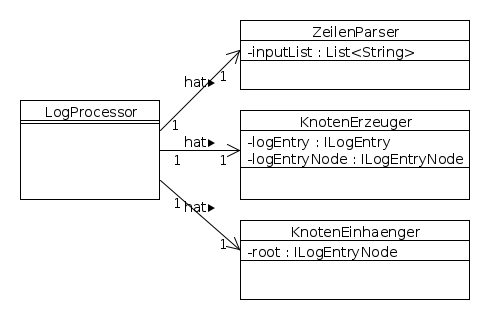
\includegraphics[width=0.6\textwidth]{Ingo/Bilder/Analyseklassendiagramm.png}
\caption{Analyseklassendiagramm Agilent-Parser}
\label{fig:Analyseklassendiagramm}
\end{figure}
\section{Entwurf}\label{Entwurf}
Ziel dieses Projektes ist es, ...

In Abbildung \ref{fig:Entwurfsklassendiagramm} auf Seite \pageref{fig:Entwurfsklassendiagramm} ist das Entwurfsklassendiagramm vom Agilent-Parser zu sehen.

\begin{figure}[htp]
\centering
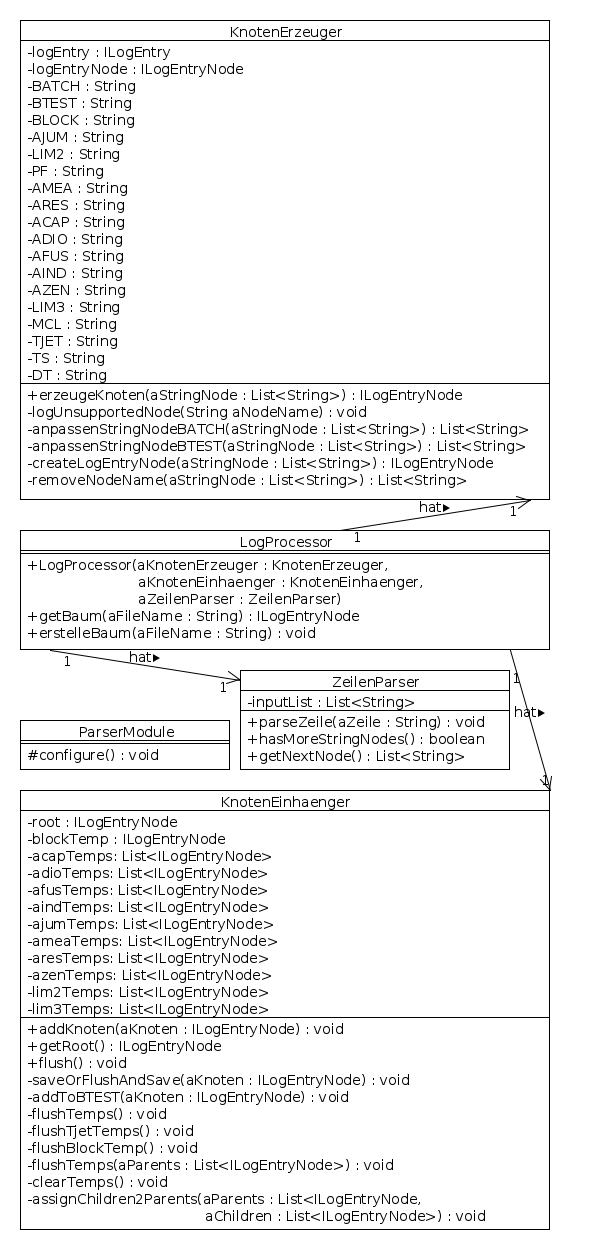
\includegraphics[width=0.6\textwidth]{Ingo/Bilder/Entwurfsklassendiagramm.png}
\caption{Entwurfsklassendiagramm Agilent-Parser}
\label{fig:Entwurfsklassendiagramm}
\end{figure}
\section{Text File Encoding}\label{TextFileEncoding}
Unter Ubuntu 10.04 ist in Eclipse Juno das Text File Encoding standartm��ig auf UTF-8 gesetzt. Die kann beim Kopieren von Stings aus dem Agilent-Logformat zu Fehlern f�hren, da bestimmte UTF-8 Zeichen im Java-Editor unsichtbar sind. Um unsichtbare Zeichen im Java-Editor sichtbar zu machen, sollte unter $Eclipse->Preference->General->Workspace$ das ``Text File Encoding'' von UTF-8 auf ISO-8859-1 umgestellt werden.
\section{Unstimmigkeiten im Agilent-Format}\label{UnstimmigkeitenImAgilentFormat}
In der Format06.pdf auf Seite 35 stimmt bei BATCH die Anzahl der Attribute nicht mit der Legende �berein. Auch in den tats�chlichen Agilent-Logdateien stimmt die Anzahl der Attribute nicht immer mit der Anzahl der Attribute �berein, wie sie in der Format06.pdf beschrieben werden.

In der Format06.pdf auf Seite 40 stimmt bei BTEST die Anzahl der Attribute nicht immer mit der tats�chlich vorkommenden Anzahl in der Agilent-Logdatei �berein.

%\chapter{Theoretische Grundlagen}
%Die f\"{u}r den Untersuchungsgegenstand relevanten Themen, die \"{u}ber die
%grundlegenden Studieninhalte hinausgehen; oft auch anwendungsspezifische Aspekte - %ca. 6 Seiten

%\chapter{Ist-Analyse}
%Welche Defizite sollen mit der Arbeit behoben werden, welche nicht? %Pr\"{a}zisierung
%der Zielstellung - ca. 6 Seiten

%\chapter{L\"{o}sungskonzept}
%Wie sollen die Defizite behoben werden? Methoden, fachliche Auseinandersetzung
%mit alternativen Ans\"{a}tzen und Auffassungen, Systembeschreibung (Architektur,
%Vorgehensmodell, \ldots) - ca. 12 Seiten

%\chapter{Implementierung}
%Umsetzung des L\"{o}sungskonzepts, Begr\"{u}ndung der verwendeten Technologien - %ca. 8
%Seiten

%\chapter{Ergebnisse}
%Objektive Bewertung der vorliegenden L\"{o}sung, diverse Testverfahren,
%Nutzerbefragungen - ca. 4 Seiten

%\chapter{Fazit und Ausblick}
%Zusammenfassung s\"{a}mtlicher Ergebnisse in Bezug auf die Zielerf\"{u}llung und
%Vorschl\"{a}ge f\"{u}r weiterf\"{u}hrende Arbeiten - ca. 2 Seiten

\bibliographystyle{alphadin}
\begin{appendix}
\newpage
\pagestyle{appendixAStyle}
%\chapter{Codebeispiele}
%\input{listings}
\end{appendix}

\newpage
\chapter{Arbeitsaufteilung}


\begin{table}[h] \begin{flushleft}  \begin{tabular}{|l||c|c|c|c|c|c|}
\hline
\textbf{Arbeit}		&	\textbf{C. Ochmann}	& \textbf{I. K�rner}  \\ \hline \hline
Abstract   	      &                     & 0       \\
Einleitung  &                             		      & ~\ref{Einleitung} \\
Aufgabenstellung&                                  & ~\ref{Aufgabenstellung}  \\
Forschungsgegenstand&                              & ~\ref{RelevanzDesForschungsgegenstandes} \\ 
akt. Wissensstand&                                      & ~\ref{DerAktuelleWissensstand}  \\ 
Hintergrund&                                      & ~\ref{Hintergrund}  \\ 
Analyse&                                      & ~\ref{Analyse}  \\ 
Funktionale Anforderungen&                                      & ~\ref{FunktionaleAnforderungen}  \\ 
Nichtfunktionale Anforderungen&                                      & ~\ref{NichtfunktionaleAnforderungen}  \\ 
Entwurf&                                      & ~\ref{Entwurf}  \\ 
Struktur und Syntax& ~\ref{strukturundsyntax} &										\\
Besonderheiten und Bemerkungen&  ~\ref{Besonderheiten}    &     \\
Entwicklungsumgebung&                                      & ~\ref{Entwicklungsumgebung}  \\ 
Dependency Injection mit Goolge Guice&                                      & ~\ref{DependencyInjectionMitGoogleGuice}  \\ 
Projekt importieren&                                      & ~\ref{ProjektImportieren}  \\ 
Projekt ausf�hren&                                      & ~\ref{ProjektAusfuehren}  \\ 
ZeilenParserTest&   ~\ref{zeilenparsertest}          &  \\
KnotenErzeugerTest&   ~\ref{knotenerzeugertest}          &  \\
KnotenEinhaengenTest&   ~\ref{knoteneinhaengentest}          &  \\
Funktionale Tests&                                      & ~\ref{FunktionaleTests}  \\ 
Zusammenfassung&                                      & ~\ref{Zusammenfassung}  \\ 
\hline \hline
\end{tabular} \end{flushleft} \caption{Aufteilung} \end{table}



\newpage
\chapter{Eigenst�ndigkeitserkl�rung}
Hiermit erkl�re ich, dass ich diese Arbeit selbst�ndig verfasst habe. Mir ist bekannt, dass jede Form des Plagiats mit der Note 5 (Betrugsversuch) bewertet wird.

\begin{tabular}{@{}p{6.0cm}p{6.0cm}}	  		  		 	
	  		 & \\
	  		 & \\
				  			\textbf{Ochmann, Christof} &               Unterschrift:\\				 
				 &\\
				 & \\
				  			\textbf{K�rner, Ingo}   	&                     Unterschrift:\\			
\end{tabular}
\end{document}
